\begin{frame}{Most Notable CNN-based Architectures}
Over time, researchers built advanced CNN architectures to improve performance and efficiency. These architectures introduced key innovations:
{\small
\begin{itemize}
    \item \textbf{LeNet \emph{[LeCun et al., 1998]}}: The first CNN architecture, designed for handwritten digit recognition.
    \item \textbf{AlexNet \emph{[Krizhevsky et al. 2012]}}:  The first CNN to achieve breakthrough performance on image classification.
    \item \textbf{VGGNet \emph{[Simonyan and Zisserman, 2014]}}: Used very deep networks (up to 19 layers).
    \item \textbf{InceptionNet (GoogLeNet) \emph{[Szegedy et al., 2014]}}: Used multiple filter sizes per layer (Inception modules).
    \item \textbf{ResNet \emph{[He et al., 2015]}}: Introduced skip connections for training very deep networks.
    \item \textbf{EfficientNet \emph{[Tan and Le, 2019]}}: Found a scaling method that  simultaneously scales a CNN’s depth, width, and resolution optimally using a single scaling coefficient.
    \item \item \textbf{MobileNet \emph{[Howard et al., 2017]}}: Designed for mobile and embedded vision applications, using depthwise separable convolutions.
\end{itemize}
}
    
\end{frame}

% LeNet-5
\begin{frame}{LeNet}
\begin{figure}
\centering
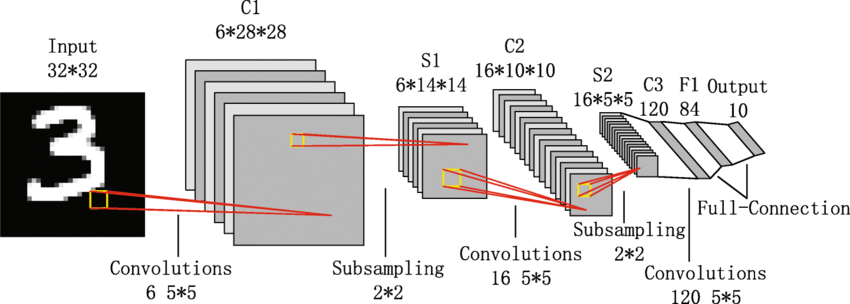
\includegraphics[width=0.8\textwidth,height=0.4\textheight,keepaspectratio]{images/cnn/lenet5.png}
\caption{LeNet-5 architecture.}
\end{figure}
{\small
\begin{itemize}
    \item LeNet-5 is a pioneering convolutional neural network (CNN) architecture developed by Yann LeCun and his collaborators in the late 1980s and early 1990s.
    \item It was primarily designed for handwritten digit recognition, specifically for the MNIST dataset.
    \item The architecture consists of two convolutional layers, followed by subsampling (pooling) layers, and then fully connected layers.
    \item It introduced key concepts such as convolutional layers, pooling layers, and the use of activation functions like sigmoid
\end{itemize}
}
\end{frame}

% AlexNet
\begin{frame}{AlexNet}
\begin{itemize}
    \item First big improvement in image classification.
    \item Made use of CNN, pooling, dropout, ReLU and training on GPUs.
    \item 5 convolutional layers, followed by max-pooling layers; with three fully connected layers at the end

\end{itemize}

\begin{figure}
\centering
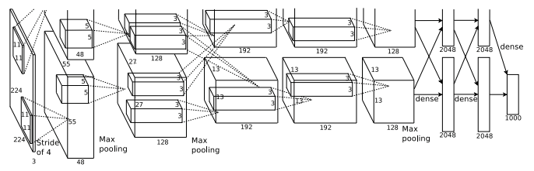
\includegraphics[width=1.0\textwidth,height=0.5\textheight,keepaspectratio]{images/cnn/alexnet.png}
\end{figure}
    
\end{frame}

% VGGNet
\begin{frame}{VGGNet}
\begin{itemize}
    \item \textbf{Improvement over AlexNet:} Uses a deeper network with small filters instead of a shallow network with larger filters.
    \item A stack of 3x3 conv layers (vs. 11x11 conv) has same receptive field, more non-linearities, fewer parameters and deeper network representation.
    \item Two variants: VGG16 or VGG19 conv layers plus 3 FC layers.
\end{itemize}

\begin{figure}
\centering
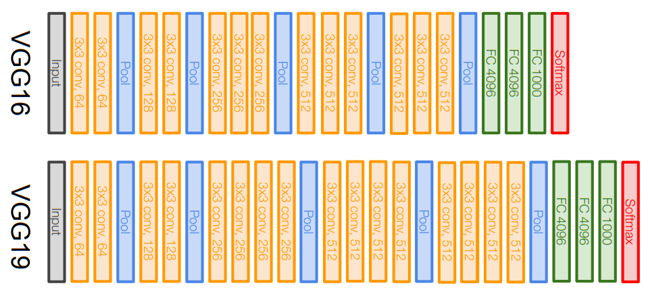
\includegraphics[width=1.0\textwidth,height=0.5\textheight,keepaspectratio]{images/cnn/VGG_16_19.png}
\end{figure}
    
\end{frame}

% InceptionNet
\begin{frame}[allowframebreaks]{InceptionNet}
    \begin{itemize}
        \item Going Deep: 22 layers
        \item Only 5 million parameters! (12× fewer than AlexNet, 27× fewer than VGGNet).
        \item Introduced efficient "Inception module"
        \item Introduced "bottleneck" layers that use 1x1 convolutions to reduce the number of channels and mix information across them.
    \end{itemize}

\begin{figure}
\centering
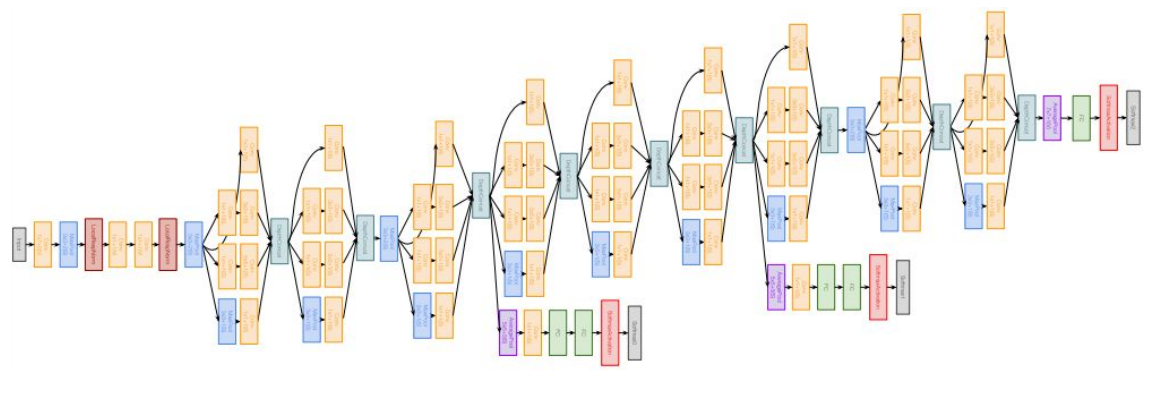
\includegraphics[width=1.0\textwidth,height=0.5\textheight,keepaspectratio]{images/cnn/inceptionnet_1.png}
\end{figure}

\framebreak

    \begin{itemize}
        \item \textbf{Inception module:} Uses multiple filter sizes (1×1, 3×3, 5×5), in parallel, to capture different features, then combines their outputs.

    \end{itemize}

\begin{figure}
\centering
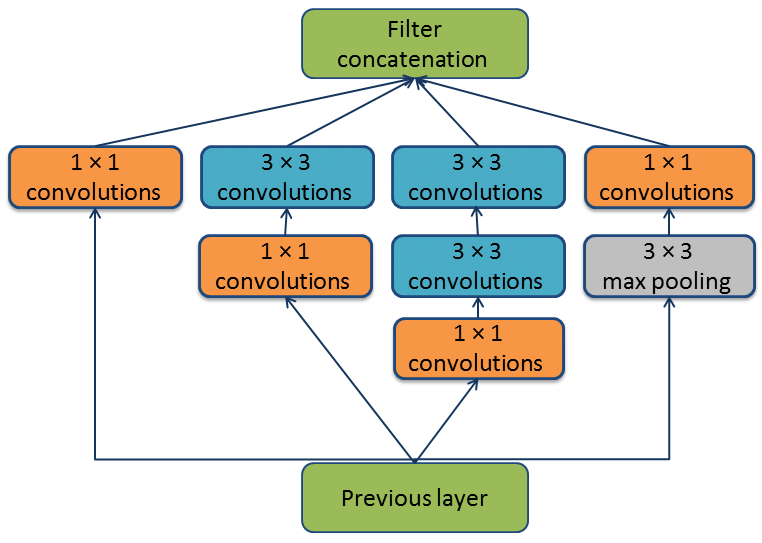
\includegraphics[width=1.0\textwidth,height=0.8\textheight,keepaspectratio]{images/cnn/inception_mod.png}
\end{figure}

\end{frame}

% ResNet
\begin{frame}{ResNet: Motivation}
\begin{itemize}
    \item \textbf{Problem:} Making networks deeper does not always improve accuracy.
    \item \textbf{Why?} In very deep networks, gradients become extremely small as they move backward through layers, making learning slow or stopping it altogether (\textbf{vanishing gradient problem}).
    \item \textbf{Solution:} Residual Network (ResNet) introduces \textbf{skip connections (residuals)}, allowing information to flow more easily.

\end{itemize}
\end{frame}

\begin{frame}{ResNet}
\begin{itemize}
    \item Very deep networks using residual connections
    \item 152-layer model for ImageNet
    \item Stacked Residual Blocks
    \item \textbf{Residual:} A shortcut connection that helps the network pass information through layers more easily.


\end{itemize}

\begin{figure}
\centering
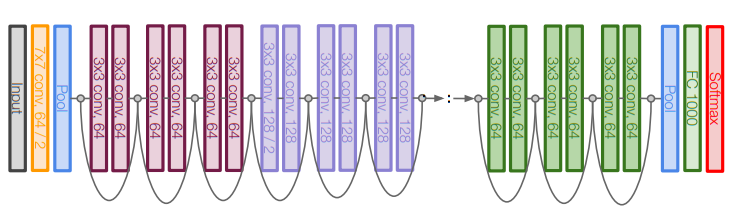
\includegraphics[width=1.0\textwidth,height=0.6\textheight,keepaspectratio]{images/cnn/resnet_1.png}
\end{figure}
\end{frame}

% EfficientNet
\begin{frame}{EfficientNet: Motivation}
\begin{itemize}
    \item \textbf{Problem:} To improve accuracy, we can:
    \begin{itemize}
        \item Increase the number of layers (\textbf{depth})
        \item Increase the number of neurons in each layer (\textbf{width})
        \item Use higher-resolution images (\textbf{resolution})
    \end{itemize}
    But finding the right balance of these three was largely based on trial and error.
    
    \item \textbf{Solution:} EfficientNet introduced a \textbf{compound scaling} method—a mathematical formula to systematically find the optimal balance among \textbf{depth}, \textbf{width}, and \textbf{resolution}.
\end{itemize}
\end{frame}

\begin{frame}{EfficientNet}

    \begin{figure}
        \centering
        % Replace with your own figure path
        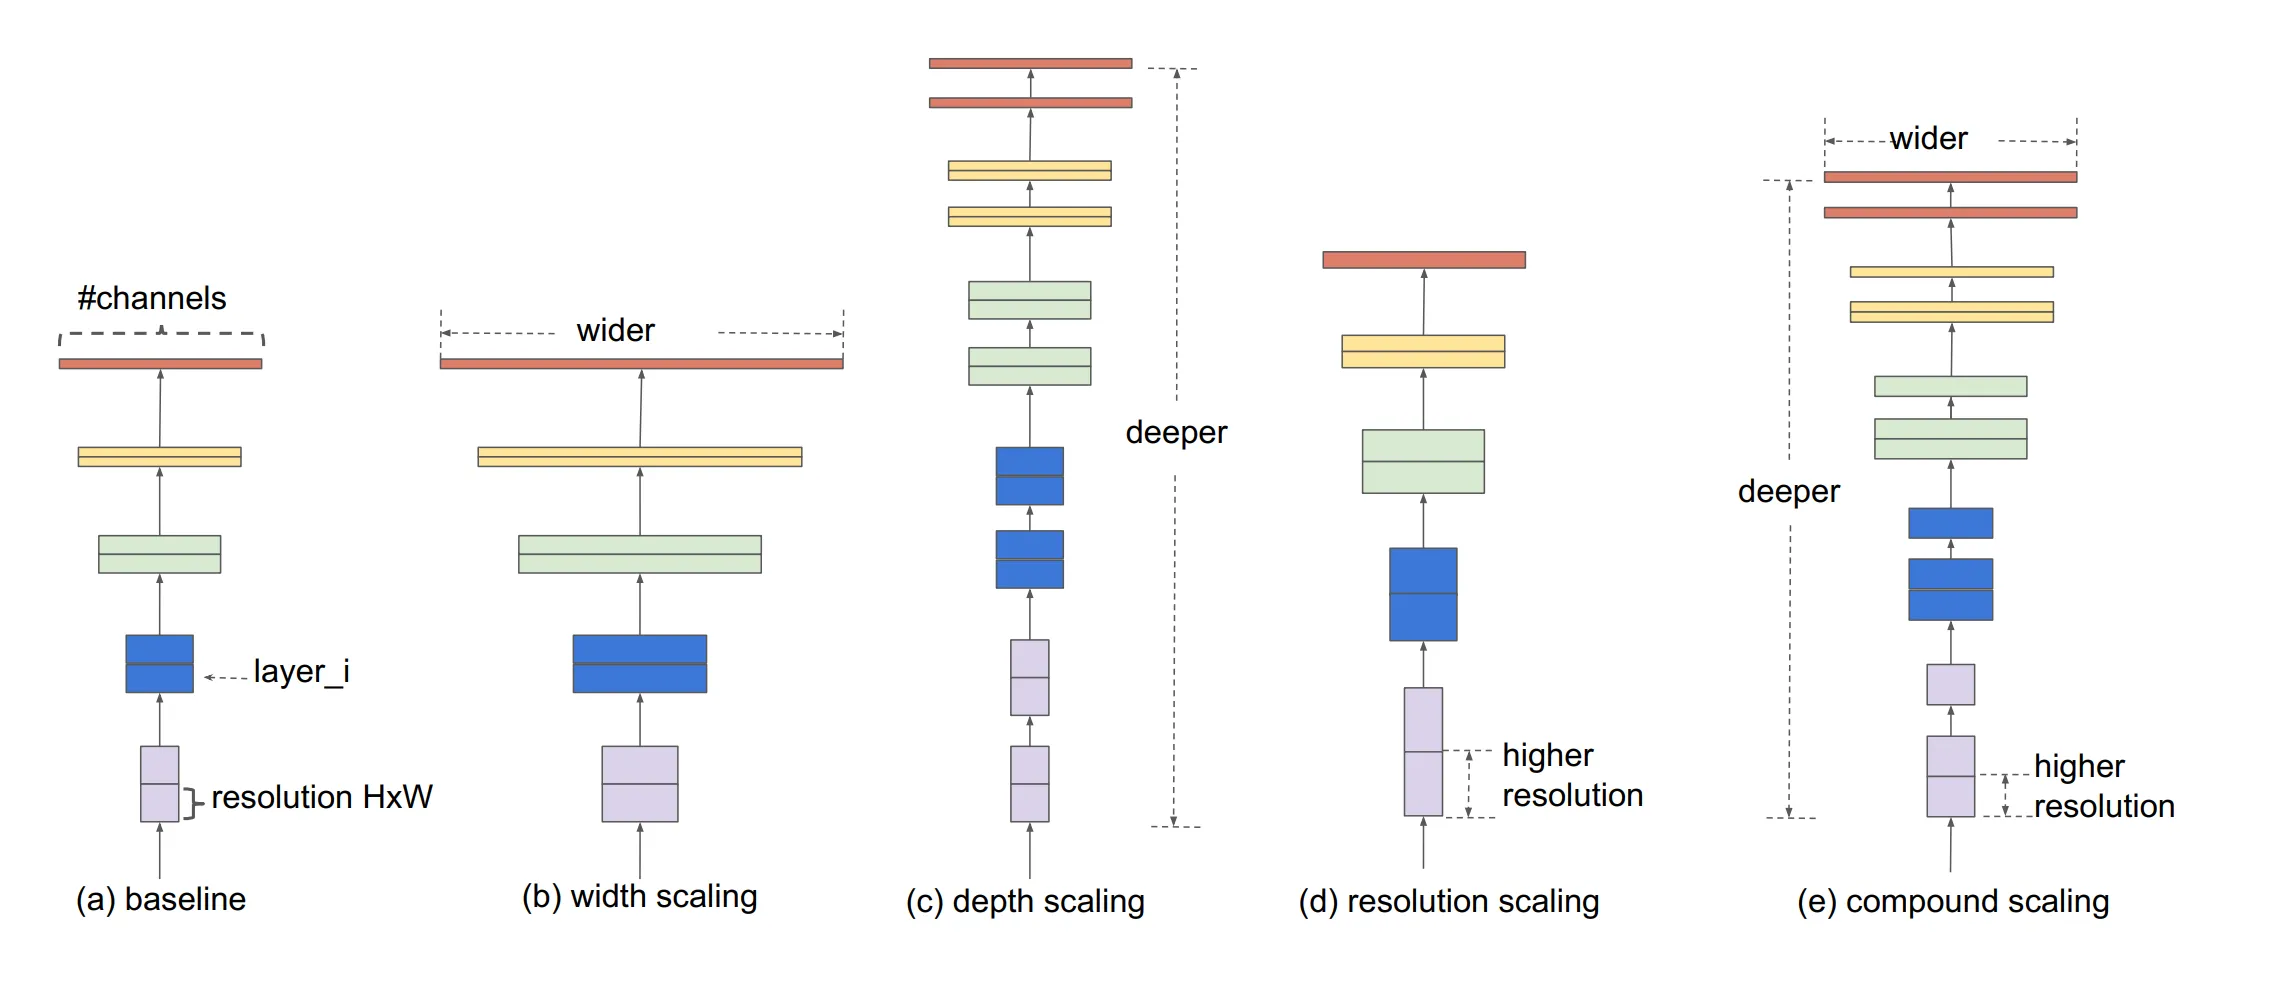
\includegraphics[width=\linewidth]{images/cnn/ENet_1.png}
        \caption{EfficientNet Scaling.}
    \end{figure}
\end{frame}


\begin{frame}{EfficientNet}
    \begin{itemize}
        \item \textbf{Compound Scaling} Uses a single \textbf{scaling coefficient} (\(\phi\)) to control:
        \begin{itemize}
        \item \textbf{Network Depth} (\(\alpha^\phi\)) → More layers
        \item \textbf{Network Width} (\(\beta^\phi\)) → More channels per layer
        \item \textbf{Input Resolution} (\(\gamma^\phi\)) → Larger input images
    \end{itemize}
        \item The goal: find \(\alpha, \beta, \gamma\) that balance accuracy \& efficiency, then scale up optimally by increasing the global coefficient \(\phi\).
    \end{itemize}

\end{frame}

\begin{frame}{EfficientNet}
\begin{itemize}
    \item EfficientNet optimizes depth, width, and resolution using this constraint:
    \[
    \alpha \cdot \beta^2 \cdot \gamma^2 \approx 2
    \]
    \item \textbf{Why this equation?}
    \begin{itemize}
        \item Increasing \textbf{depth} (\(\alpha\)) increases FLOPs \textbf{linearly}.
        \item Increasing \textbf{width} (\(\beta\)) increases FLOPs \textbf{quadratically} (\(\beta^2\)).
        \item Increasing \textbf{resolution} (\(\gamma\)) increases FLOPs \textbf{quadratically} (\(\gamma^2\)).
    \end{itemize}
    \item To double total FLOPs, the three factors must be balanced together.
\end{itemize}
\end{frame}



\begin{frame}{EfficientNet}
\begin{itemize}
    \item The authors of EfficientNet searched for the best scaling factors on a small baseline model.
    \item They found:
    \[
    \alpha = 1.2, \quad \beta = 1.1, \quad \gamma = 1.15
    \]
\end{itemize}
\end{frame}

\begin{frame}{EfficientNet Scaling: B0 to B7}
\begin{itemize}
    \item The EfficientNet family (B0 to B7) is generated using:
    \[
    \text{Depth} = 1.2^\phi, \quad
    \text{Width} = 1.1^\phi, \quad
    \text{Resolution} = 1.15^\phi
    \]
\end{itemize}

\begin{table}[]
    \centering
    \begin{tabular}{|c|c|c|c|}
        \hline
        \textbf{Model} & \(\phi\) & \textbf{Depth} (\(\alpha^\phi\)) & \textbf{Width} (\(\beta^\phi\)) \\ 
        \hline
        B0 & 0 & \(1.2^0 = 1.0\) & \(1.1^0 = 1.0\)  \\ 
        B1 & 1 & \(1.2^1 = 1.2\) & \(1.1^1 = 1.1\)  \\ 
        B2 & 2 & \(1.2^2 = 1.44\) & \(1.1^2 = 1.21\)  \\ 
        B3 & 3 & \(1.2^3 = 1.73\) & \(1.1^3 = 1.33\)  \\ 
        B4 & 4 & \(1.2^4 = 2.07\) & \(1.1^4 = 1.46\)  \\ 
        B5 & 5 & \(1.2^5 = 2.49\) & \(1.1^5 = 1.61\)  \\ 
        B6 & 6 & \(1.2^6 = 2.99\) & \(1.1^6 = 1.77\)  \\ 
        B7 & 7 & \(1.2^7 = 3.58\) & \(1.1^7 = 1.94\)  \\ 
        \hline
    \end{tabular}
    \caption{Scaling EfficientNet from B0 to B7}
\end{table}

\begin{itemize}
\item We multiply these scaling factors by the baseline EfficientNet-B0 values and round to the nearest integer to get the new depth, width, and resolution for each model.
\end{itemize}


\end{frame}


\begin{frame}{EfficientNet}

\begin{itemize}
    \item EfficientNet models achieve state-of-the-art accuracy with significantly fewer parameters and FLOPs.        \pause

    \item EfficientNet-B7 reaches 84.4\% Top-1 and 97.3\% Top-5 accuracy on ImageNet.
    \pause

    \item More efficient than previous CNN models---8.4x smaller and 6.1x faster than competitors.
\end{itemize}
\end{frame}


\begin{frame}{EfficientNet Performance}
\begin{figure}
\centering
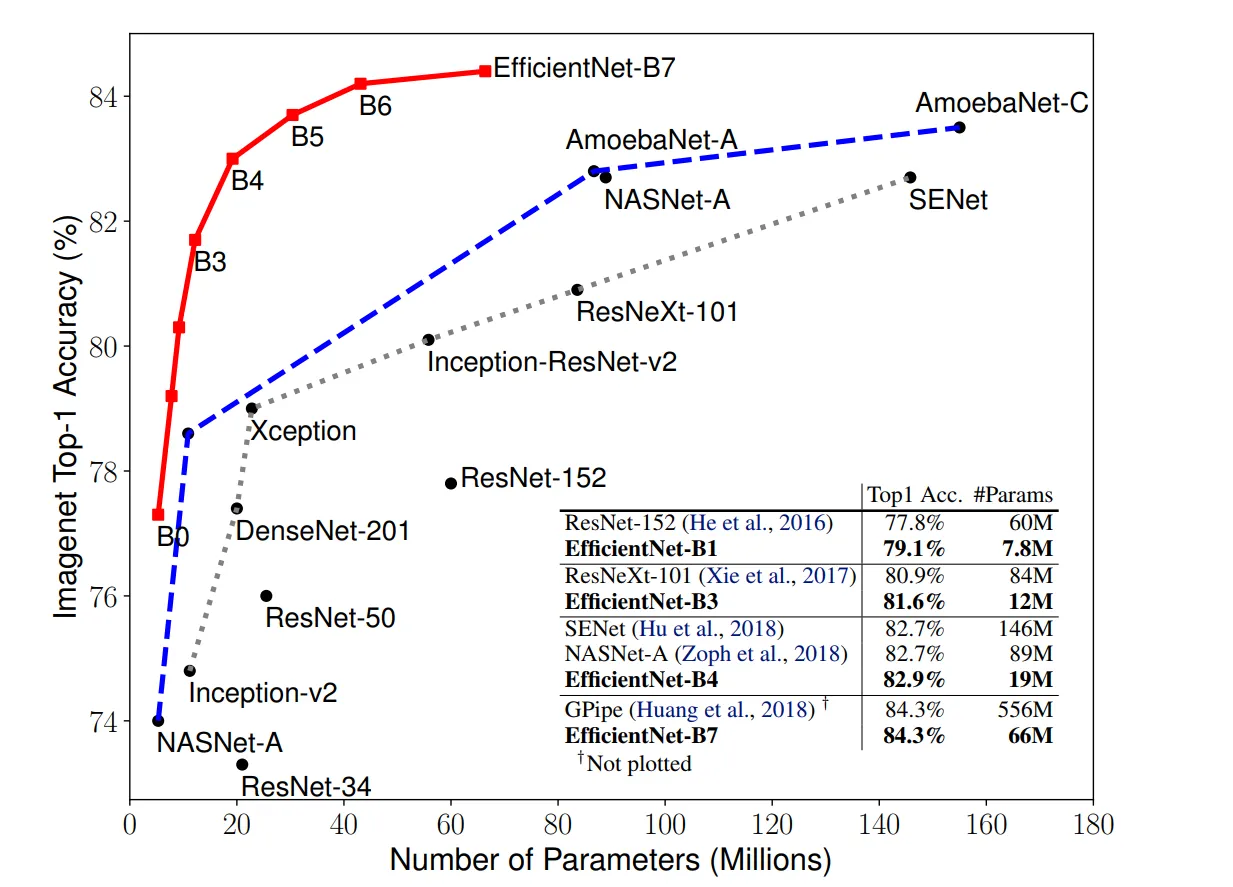
\includegraphics[width=\textwidth,height=.7\textheight,keepaspectratio]{images/cnn/ENet_2.png}
\caption{EfficientNet Performance on Imagenet.}
\end{figure}
\end{frame}

% MobileNet
\begin{frame}{Motivation for MobileNets}
\begin{itemize}
    \item \textbf{Why MobileNets?}
    \begin{itemize}
        \item Small-sized models are crucial for mobile and embedded devices.
        \item MobileNets reduce computational cost and memory usage while maintaining good accuracy.
    \end{itemize}
    \item \textbf{Key Idea:}
    \begin{itemize}
        \item Use \textbf{depthwise-separable convolutions} to significantly reduce computation compared to standard convolutions.
    \end{itemize}
\end{itemize}
\end{frame}

\begin{frame}{Computational Cost of Convolutions}
\begin{itemize}
    \item \textbf{Computational cost of standard convolution:}
    \[
    \text{Cost} = \text{\# filter params} \times \text{\# filter positions} \times \text{\# filters}
    \]
    \item Filters operate on all input channels, increasing computation significantly.
\end{itemize}
\begin{figure}
    \centering
    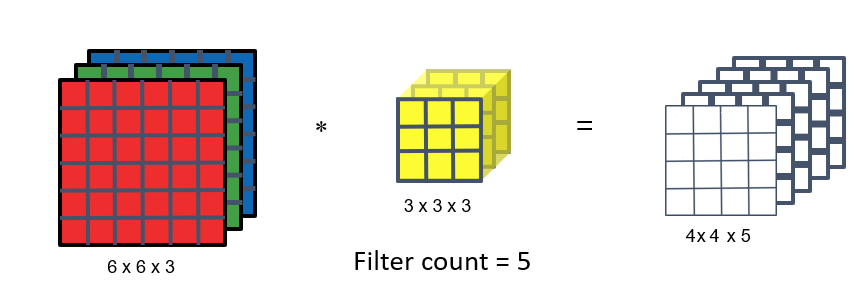
\includegraphics[width=0.8\linewidth]{images/cnn/NormalConv_MobileNet.png} 
\end{figure}
\end{frame}

\begin{frame}{Depthwise-Separable Convolutions}
\begin{itemize}
    \item Split standard convolution into two steps:
    \begin{itemize}
        \item \textbf{Depthwise Convolution:} Applies a single filter per input channel.
        \item \textbf{Pointwise Convolution:} Combines outputs from depthwise convolution.
    \end{itemize}
    \item \textbf{Key Benefit:} Reduces computational cost significantly compared to standard convolution.
\end{itemize}
\begin{figure}
    \centering
    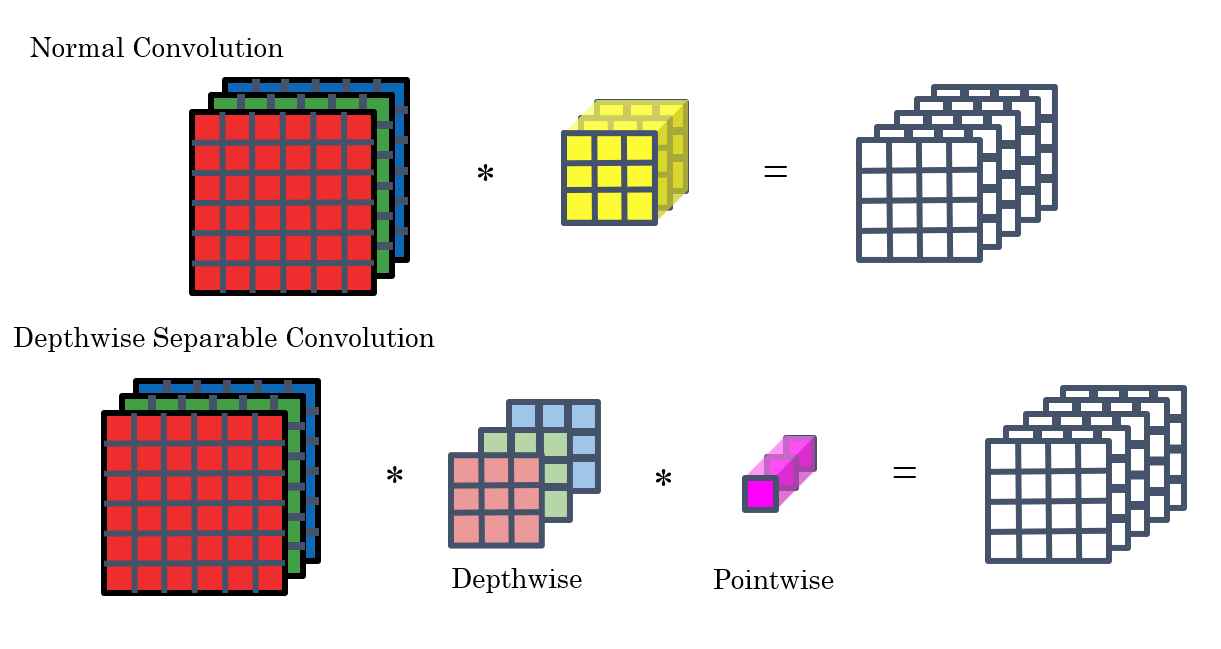
\includegraphics[width=0.8\linewidth]{images/cnn/Depth_vs_Normal_Conv.png} 
\end{figure}
\end{frame}

\begin{frame}{Depthwise Convolution}
\begin{itemize}
    \item Operates on each input channel separately.
\end{itemize}
\begin{figure}
    \centering
    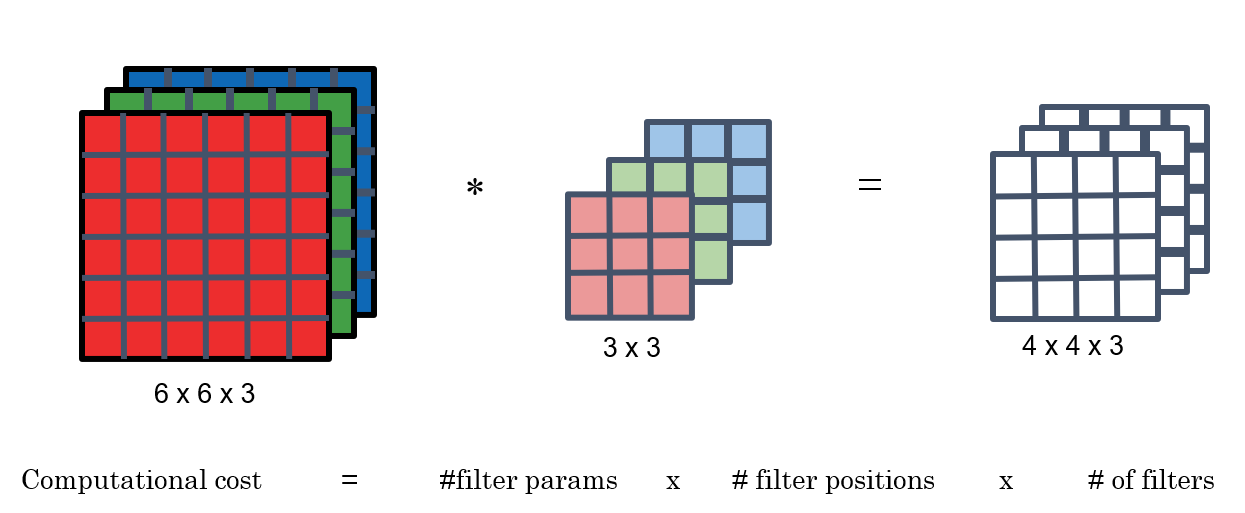
\includegraphics[width=0.8\linewidth]{images/cnn/Depthwise_conv.png}
\end{figure}
\end{frame}


\begin{frame}{Pointwise Convolution}
\begin{itemize}
    \item Combines outputs from depthwise convolution using \(1 \times 1\) convolutions (mixes channels).
\end{itemize}
\begin{figure}
    \centering
    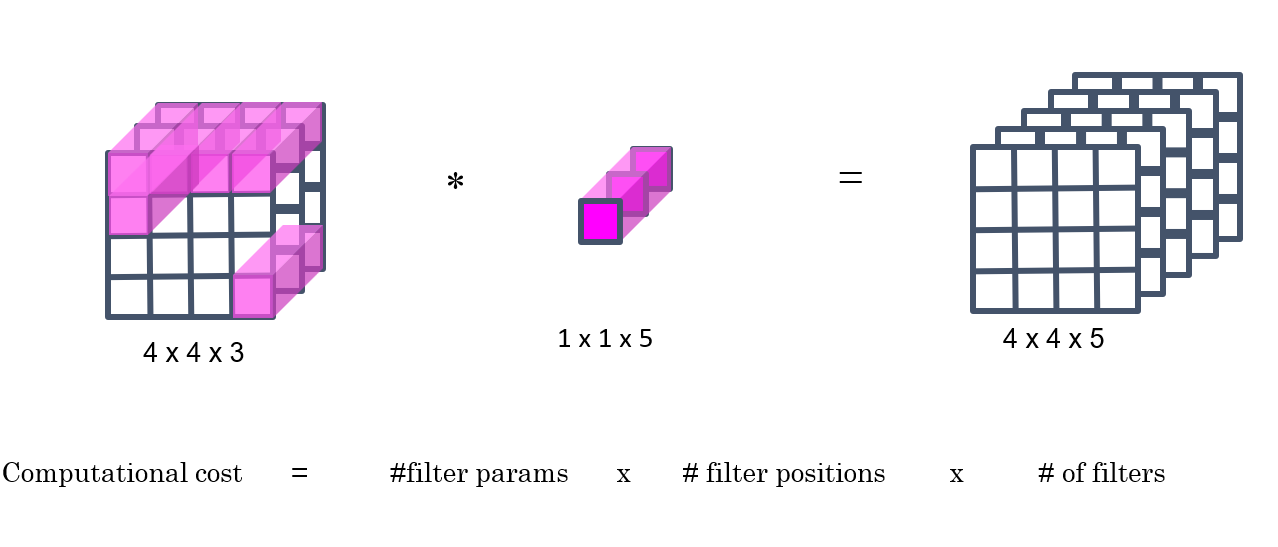
\includegraphics[width=0.8\linewidth]{images/cnn/PointWise_conv.png}
\end{figure}
\end{frame}

\begin{frame}{MobileNet Architectures}
\begin{itemize}
    \item \textbf{MobileNet v2:}
    \begin{itemize}
        \item Adds \textbf{residual connections}.
        \item Introduces:
        \begin{itemize}
            \item \textbf{Expansion step:} Expands input dimensions before depthwise convolution.
            \item \textbf{Projection step:} Reduces dimensions after processing.
        \end{itemize}
    \end{itemize}
\end{itemize}
\begin{figure}
    \centering
    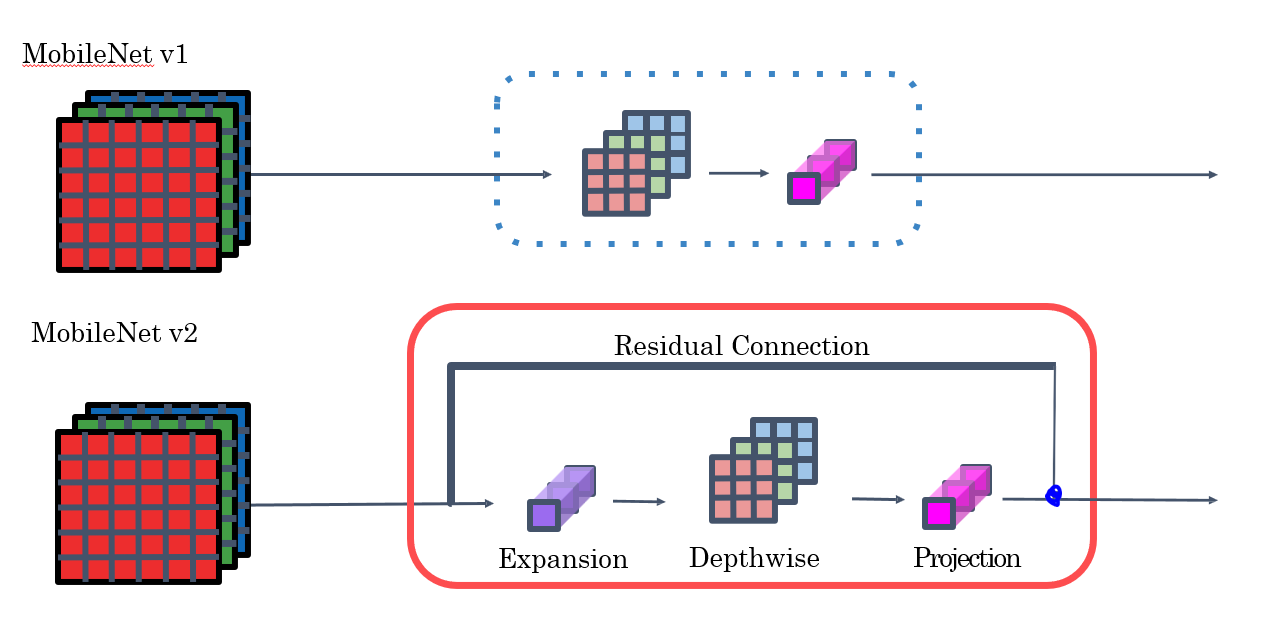
\includegraphics[width=0.8\textwidth,height=.7\textheight,keepaspectratio]{images/cnn/MobileNet_1_and_2.png} 
\end{figure}
\end{frame}
